% Pengaturan ukuran teks dan jenis dokumen
\documentclass[12pt]{report}

% Pengaturan ukuran halaman dan margin
\usepackage[a4paper,top=30mm,left=30mm,right=20mm,bottom=20mm]{geometry}

% Pengaturan ukuran spasi
\usepackage[singlespacing]{setspace}

% Judul dokumen
\title{Proposal Tugas Akhir ITS}
\author{Musk, Elon Reeve}

% Pengaturan format bahasa
\usepackage[indonesian]{babel}

% Pengaturan detail pada file PDF
\usepackage[pdfauthor={\@author},bookmarksnumbered,pdfborder={0 0 0}]{hyperref}

% Pengaturan jenis karakter
\usepackage[utf8]{inputenc}

% Package lainnya
\usepackage{etoolbox} % Mengubah fungsi default
\usepackage{enumitem} % Pembuatan list
\usepackage{lipsum} % Pembuatan template kalimat
\usepackage{graphicx} % Input gambar
\usepackage{longtable} % Pembuatan tabel
\usepackage[table,xcdraw]{xcolor} % Pewarnaan tabel
\usepackage[sectionbib]{natbib} % Kutipan artikel
\usepackage{changepage} % Pembuatan teks kolom
\usepackage{multicol} % Pembuatan kolom ganda
\usepackage{multirow} % Pembuatan baris ganda

% Pengaturan format judul bab
\usepackage{titlesec}
\renewcommand{\thesection}{\arabic{section}}
\titleformat*{\section}{\normalsize\bfseries}
\titleformat*{\subsection}{\normalsize\bfseries}
\titlespacing{\section}{0ex}{3ex}{1.5ex}
\titlespacing{\subsection}{0ex}{3ex}{1.5ex}

% Isi keseluruhan dokumen
\begin{document}

  % Menonaktifkan penomoran halaman
  \pagenumbering{gobble}

  % Lembar pengesahan
  \begin{flushleft}
  % Ubah kalimat berikut sesuai dengan nama departemen dan fakultas
  \textbf{Departemen Teknik Dirgantara - FTD}\\
  % Ubah kalimat berikut sesuai dengan nama universitas
  \textbf{Institut Teknologi Sepuluh Nopember}\\
\end{flushleft}

\begin{center}
  % Ubah detail mata kuliah berikut sesuai dengan yang ditentukan oleh departemen
  \underline{\textbf{TD123456 - PRA TUGAS AKHIR - 2 SKS}}
\end{center}

\begin{adjustwidth}{-0.2cm}{}
  \begin{tabular}{lcp{0.7\linewidth}}

    % Ubah kalimat-kalimat berikut sesuai dengan nama dan NRP mahasiswa
    Nama Mahasiswa &:& Elon Reeve Musk \\
    Nomor Pokok &:&	0123 20 4000 0001 \\

    % Ubah kalimat berikut sesuai dengan semester pengajuan proposal
    Semester &:& Genap 2019/2020 \\

    % Ubah kalimat-kalimat berikut sesuai dengan nama-nama dosen pembimbing
    Calon Dosen Pembimbing &:& 1. Nikola Tesla, S.T., M.T. \\
    & & 2. Wernher von Braun, S.T., M.T. \\

    % Ubah kalimat berikut sesuai dengan judul tugas akhir
    Judul Tugas Akhir &:& \textbf{Kalkulasi Energi pada Roket Luar Angkasa Berbasis Anti Gravitasi} \\

    Uraian Tugas Akhir &:& \\
  \end{tabular}
\end{adjustwidth}

% Ubah paragraf berikut sesuai dengan uraian dari tugas akhir
Pesatnya perkembangan roket yang merupakan \lipsum[1]
\vspace{1ex}

\begin{flushright}
  % Ubah kalimat berikut sesuai dengan tempat, bulan, dan tahun penulisan
  Surabaya, 2 Maret 2020
\end{flushright}
\vspace{1ex}

\begin{center}

  \begin{multicols}{2}

    Dosen Pembimbing 1
    \vspace{12ex}

    % Ubah kalimat-kalimat berikut sesuai dengan nama dan NIP dosen pembimbing pertama
    \underline{Nikola Tesla, S.T., M.T.} \\
    NIP. 18560710 194301 1 001

    \columnbreak

    Dosen Pembimbing 2
    \vspace{12ex}

    % Ubah kalimat-kalimat berikut sesuai dengan nama dan NIP dosen pembimbing kedua
    \underline{Wernher von Braun, S.T., M.T.} \\
    NIP. 19230323 197706 1 001

  \end{multicols}
  \vspace{6ex}

  Mengetahui, \\
  % Ubah kalimat berikut sesuai dengan jabatan kepala departemen
  Kepala Departemen Teknik Dirgantara FTD - ITS
  \vspace{12ex}

  % Ubah kalimat-kalimat berikut sesuai dengan nama dan NIP kepala departemen
  \underline{Dr. Leonardo Da Vinci, S.T., M.T.} \\
  NIP. 14520415 151905 1 001

\end{center}

  \newpage

  % Konten pendahuluan
  \chapter{PENDAHULUAN}

\section{Latar Belakang}

% Ubah paragraf-paragraf berikut sesuai dengan latar belakang dari tugas akhir
Pesatnya perkembangan roket yang merupakan \lipsum[2]

\lipsum[3]

\section{Rumusan Masalah}

% Ubah paragraf berikut sesuai dengan rumusan masalah dari tugas akhir
Berdasarkan hal yang telah dipaparkan di latar belakang, \lipsum[4]

\section{Batasan Masalah atau Ruang Lingkup}

\lipsum[6]

\section{Tujuan}

% Ubah paragraf berikut sesuai dengan tujuan penelitian dari tugas akhir
Tujuan dari penelitian ini adalah \lipsum[7][1-14]

\section{Manfaat}

% Ubah paragraf berikut sesuai dengan tujuan penelitian dari tugas akhir
Manfaat dari penelitian ini adalah \lipsum[8][1-14]


  % Konten tinjauan pustaka
  \section{TINJAUAN PUSTAKA}

% Ubah konten-konten berikut sesuai dengan isi dari tinjauan pustaka

\subsection{Roket Luar Angkasa}

% Contoh input gambar dengan format *.jpg
\begin{figure} [ht] \centering
  % Nama dari file gambar yang diinputkan
	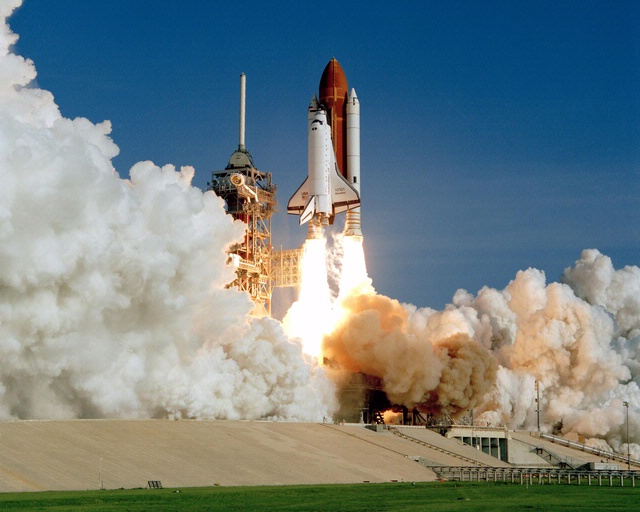
\includegraphics[scale=0.45]{gambar/space-shuttle.jpg}
  % Keterangan gambar yang diinputkan
	\caption{Peluncuran Pesawat Luar Angkasa \emph{Discovery}}
  % Label referensi dari gambar yang diinputkan
	\label{fig:spaceShuttle}
\end{figure}

% Contoh penggunaan referensi dari gambar yang diinputkan
\emph{Discovery} \ref{fig:spaceShuttle} merupakan \lipsum[2]

\subsection{Hukum Newton}

% Contoh penggunaan referensi dari pustaka
Newton pernah merumuskan \citep{newtonLaw} bahwa \lipsum[2]
% Contoh penggunaan referensi dari persamaan
Kemudian menjadi persamaan seperti pada persamaan \ref{eq:hukumPertama}.

% Contoh pembuatan persamaan
\begin{equation}
  % Label referensi dari persamaan yang dibuat
  \label{eq:hukumPertama}
  % Baris kode persamaan yang dibuat
  \sum \mathbf{F} = 0\; \Leftrightarrow\; \frac{\mathrm{d} \mathbf{v} }{\mathrm{d}t} = 0.
\end{equation}

  % Konten metodologi
  \section{METODOLOGI}

% Ubah konten-konten berikut sesuai dengan isi dari metodologi

\subsection{Metode yang digunakan}

\lipsum[11]

% Contoh input gambar dengan format *.jpg
\begin{figure} [ht] \centering
  % Nama dari file gambar yang diinputkan
  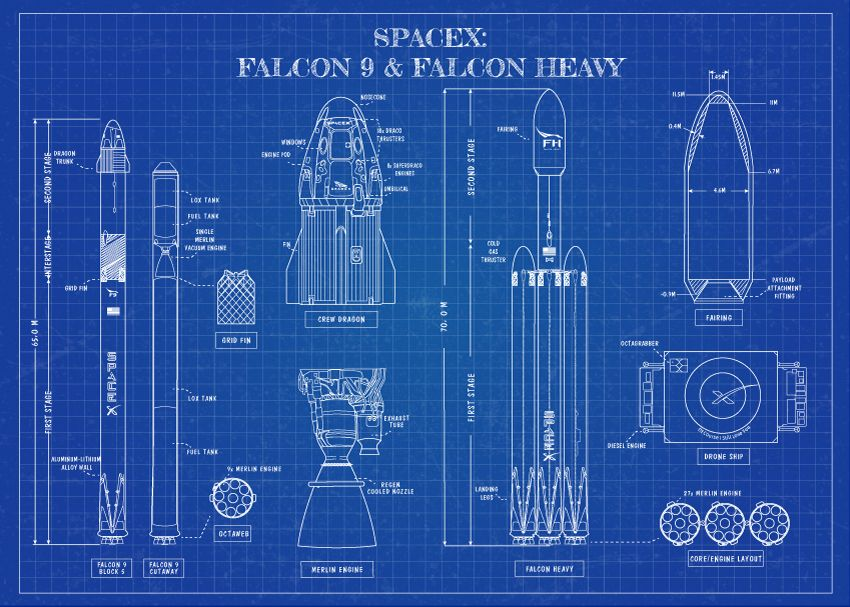
\includegraphics[scale=0.45]{gambar/blueprint.jpg}
  % Keterangan gambar yang diinputkan
  \caption{\emph{Blueprint} roket yang akan diuji coba \parencite{SpaceXBlueprint}}
  % Label referensi dari gambar yang diinputkan
  \label{fig:Blueprint}
\end{figure}

% Contoh penggunaan referensi dari gambar yang diinputkan
Pada \emph{blueprint} yang tertera di Gambar \ref{fig:Blueprint}. \lipsum[12]

\subsection{Bahan dan peralatan yang digunakan}

\lipsum[13]
\lipsum[3]

\subsection{Urutan pelaksanaan penelitian}

% Ubah tabel berikut sesuai dengan isi dari rencana kerja
\newcommand{\w}{}
\newcommand{\G}{\cellcolor{gray}}
\begin{table}[h!]
  \begin{tabular}{|p{3.5cm}|c|c|c|c|c|c|c|c|c|c|c|c|c|c|c|c|}

    \hline
    \multirow{2}{*}{Kegiatan} & \multicolumn{16}{|c|}{Minggu} \\
    \cline{2-17} &
    1 & 2 & 3 & 4 & 5 & 6 & 7 & 8 & 9 & 10 & 11 & 12 & 13 & 14 & 15 & 16 \\
    \hline

    % Gunakan \G untuk mengisi sel dan \w untuk mengosongkan sel
    Pengambilan data &
    \G & \G & \G & \G & \w & \w & \w & \w & \w & \w & \w & \w & \w & \w & \w & \w \\
    \hline

    Pengolahan data &
    \w & \w & \w & \w & \G & \G & \G & \G & \w & \w & \w & \w & \w & \w & \w & \w \\
    \hline

    Analisa data &
    \w & \w & \w & \w & \w & \w & \w & \w & \G & \G & \G & \G & \w & \w & \w & \w \\
    \hline

    Evaluasi penelitian &
    \w & \w & \w & \w & \w & \w & \w & \w & \w & \w & \w & \w & \G & \G & \G & \G \\
    \hline

  \end{tabular}
  \captionof{table}{Tabel timeline}
  \label{tbl:timeline}
\end{table}

Pada \emph{timeline} yang tertera di Tabel \ref{tbl:timeline} \lipsum[10]


  % Konten lainnya
  \section{HASIL YANG DIHARAPKAN}

Dari penelitian yang akan dilakukan, diharapkan \lipsum[13]

\section{RENCANA KERJA}

% Ubah tabel berikut sesuai dengan isi dari rencana kerja
\newcommand{\w}{}
\newcommand{\G}{\cellcolor{gray}}
\begin{table}[h!]
  \begin{tabular}{|p{3.5cm}|c|c|c|c|c|c|c|c|c|c|c|c|c|c|c|c|}

    \hline
    \multirow{2}{*}{Kegiatan} & \multicolumn{16}{|c|}{Minggu} \\
    \cline{2-17} &
    1 & 2 & 3 & 4 & 5 & 6 & 7 & 8 & 9 & 10 & 11 & 12 & 13 & 14 & 15 & 16 \\
    \hline

    % Gunakan \G untuk mengisi sel dan \w untuk mengosongkan sel
    Pengambilan data &
    \G & \G & \G & \G & \w & \w & \w & \w & \w & \w & \w & \w & \w & \w & \w & \w \\
    \hline

    Pengolahan data &
    \w & \w & \w & \w & \G & \G & \G & \G & \w & \w & \w & \w & \w & \w & \w & \w \\
    \hline

    Analisa data &
    \w & \w & \w & \w & \w & \w & \w & \w & \G & \G & \G & \G & \w & \w & \w & \w \\
    \hline

    Evaluasi penelitian &
    \w & \w & \w & \w & \w & \w & \w & \w & \w & \w & \w & \w & \G & \G & \G & \G \\
    \hline

    Penyusunan laporan &
    \G & \G & \G & \G & \G & \G & \G & \G & \G & \G & \G & \G & \G & \G & \G & \G \\
    \hline

  \end{tabular}
\end{table}

  % Daftar pustaka
  \section{DAFTAR PUSTAKA}
  \renewcommand\bibname{}
  \vspace{-2ex}
  \bibliographystyle{plain}
  \bibliography{pustaka/pustaka.bib}

\end{document}